% $Header: /cvsroot/latex-beamer/latex-beamer/solutions/conference-talks/conference-ornate-20min.en.tex,v 1.6 2004/10/07 20:53:08 tantau Exp $

\documentclass{beamer}

\mode<presentation>
{
%  \usetheme{Hannover}
\usetheme[width=0.7in]{Hannover}
% or ...

  \setbeamercovered{transparent}
  % or whatever (possibly just delete it)
}
\usepackage{longtable}
\usepackage{booktabs}
\usepackage{qtree}

\usepackage[english]{babel}
% or whatever

\usepackage[latin1]{inputenc}
% or whatever

\usepackage{times}
%\usepackage[T1]{fontenc}
% Or whatever. Note that the encoding and the font should match. If T1
% does not look nice, try deleting the line with the fontenc.
%\usepackage{logictheme}

%\usepackage{hhline}
\usepackage{multirow}
%\usepackage{multicol}
%\usepackage{array}
%\usepackage{supertabular}
%\usepackage{amsmath}
%\usepackage{amsfonts}
\usepackage{totpages}
\usepackage{hyperref}
%\usepackage{booktabs}

%\usepackage{bm}

\usepackage{listings}
\usepackage{tikz}
\newcommand{\blt}{- } %used for bullets in a list

\newcounter{datadefnum} %Datadefinition Number
\newcommand{\ddthedatadefnum}{DD\thedatadefnum}
\newcommand{\ddref}[1]{DD\ref{#1}}

\newcommand{\colAwidth}{0.2\textwidth}
\newcommand{\colBwidth}{0.73\textwidth}

\renewcommand{\arraystretch}{0.6} %so that tables with equations do not look crowded

\pgfdeclareimage[height=0.7cm]{logo}{McMasterLogo}
\title[\pgfuseimage{logo}]  % (optional, use only with long paper titles)
{Literate Scientific Software \&\\ The Drasil Framework}

%\subtitle
%{Include Only If Paper Has a Subtitle}

\author[Slide \thepage~of \pageref{TotPages}] % (optional, use only with lots of
                                              % authors)
{Dan Szymczak}
% - Give the names in the same order as the appear in the paper.
% - Use the \inst{?} command only if the authors have different
%   affiliation.

\institute[McMaster University] % (optional, but mostly needed)
{
  Computing and Software Department\\
  Faculty of Engineering\\
  McMaster University
}
% - Use the \inst command only if there are several affiliations.
% - Keep it simple, no one is interested in your street address.

\date[Jan 12, 2016] % (optional, should be abbreviation of conference name)
{Ernie Mileta Visit, Feb.\ 28, 2017}
% - Either use conference name or its abbreviation.
% - Not really informative to the audience, more for people (including
%   yourself) who are reading the slides online

\subject{computational science and engineering, software engineering, software
  quality, literate programming, software requirements specification, document
  driven design}
% This is only inserted into the PDF information catalog. Can be left
% out. 

% If you have a file called "university-logo-filename.xxx", where xxx
% is a graphic format that can be processed by latex or pdflatex,
% resp., then you can add a logo as follows:

%\pgfdeclareimage[height=0.5cm]{Mac-logo}{McMasterLogo}
%\logo{\pgfuseimage{Mac-logo}}

% Delete this, if you do not want the table of contents to pop up at
% the beginning of each subsection:
\AtBeginSubsection[]
{
  \begin{frame}<beamer>
    \frametitle{Outline}
    \tableofcontents[currentsection,currentsubsection]
  \end{frame}
}

% If you wish to uncover everything in a step-wise fashion, uncomment
% the following command: 

%\beamerdefaultoverlayspecification{<+->}

\beamertemplatenavigationsymbolsempty 

% have SRS and LP open during the presentation

\begin{document}

%%%%%%%%%%%%%%%%%%%%%%%%%%%%%%%%%%%%%%
\begin{frame}

\titlepage

\end{frame}

%%%%%%%%%%%%%%%%%%%%%%%%%%%%%%%%%%%%%%

\begin{frame}

\frametitle{Overview}
\tableofcontents
% You might wish to add the option [pausesections]

% make like a story - the phases - reason for, why works, advantages
% changing the history a bit to make a more rational narrative

\end{frame}

%%%%%%%%%%%%%%%%%%%%%%%%%%%%%%%%%%%%%%

\section[LSS]{Literate Scientific Software}

% \subsection[Important Software Qualities]{Scientific Computing Software
% Qualities}

%%%%%%%%%%%%%%%%%%%%%%%%%%%%%%%%%%%%%%

\begin{frame}

\frametitle{Literate Scientific Software}

\begin{itemize}
\item Motivation
\begin{itemize}
\item Improve verifiability, maintainability and reusability.
\item Save money and time% when managing change.
\end{itemize}
\item One ``source,'' multiple views
\begin{itemize}
\item Requirements%, including or excluding derivations.
\item Design
\item Test Cases
\item Build instructions
\item ...
\end{itemize}
\end{itemize}
\end{frame}

%%%%%%%%%%%%%%%%%%%%%%%%%%%%%%%%%%%%%%

\begin{frame}[label=motivation]

\frametitle{Motivation}
\begin{center}
\begin{tikzpicture}[node distance=5mm]
  \tikzstyle{every node}=[draw,shape=rectangle, rounded corners,
    text width=7em, text centered];
  \node (srs) at (-4,0)         	{Requirements};
  \node (dd) at (-3.5,-1.2)  {\alert<3>{Design}};
  \node (src) at (-3,-2.4) 	{\alert<3>{Code}};
  \node (test) at (-2.5, -3.6)       {\alert<3>{Testing}};
\only<2-3>{\node(change) at (0,0) {Change R1};};
	\alt<2-3>{\draw [gray, ->, line width=2pt] (srs) -- (dd);}
  		{\draw [->, line width=2pt] (srs) -- (dd);}
  	\alt<2-3>{\draw [gray, ->, line width=2pt] (dd) -- (src);}
		{\draw [->, line width=2pt] (dd) -- (src);}
  	\alt<2-3>{\draw [gray, ->, line width=2pt] (src) -- (test);}
  		{\draw [->, line width=2pt] (src) -- (test);}
  \only<2-3>{
	\alt<3>{\draw [gray, ->, line width = 3pt] (srs) -- (change);}
		{\draw [->, line width = 3pt] (srs) -- (change);}
	}
  \only<3>{
	\draw [red, ->, line width = 3pt] (change) -- (dd);
	\draw [red, ->, line width = 3pt] (change) -- (src);
	\draw [red, ->, line width = 3pt] (change) -- (test);
	};
\end{tikzpicture}
\end{center}

\end{frame}

%%%%%%%%%%%%%%%%%%%%%%%%%%%%%%%%%%%%%%

\begin{frame}

\frametitle{Last Time}
\begin{itemize}
\item Toy example
\item ``Recipes'', ``chunks'', and \textit{knowledge capture}
\item Common/specific knowledge
\item Drasil design
\end{itemize}

\end{frame}

%%%%%%%%%%%%%%%%%%%%%%%%%%%%%%%%%%%%%%

\begin{frame}

\frametitle{Recap - Knowledge Capture}
\begin{center}
\includegraphics[width=.6\textwidth]{KC.jpg}
\end{center}

\end{frame}

%%%%%%%%%%%%%%%%%%%%%%%%%%%%%%%%%%%%%%

\begin{frame}

\frametitle{Recap - Generation}
\begin{center}
\includegraphics[width=.6\textwidth]{generate_all_the_things.jpg}
\end{center}

\end{frame}

%%%%%%%%%%%%%%%%%%%%%%%%%%%%%%%%%%%%%%

\section[Drasil]{Drasil Today}

%%%%%%%%%%%%%%%%%%%%%%%%%%%%%%%%%%%%%%

\begin{frame}

\frametitle{Drasil}
\begin{center}
\includegraphics[width=.65\textwidth]{tree.png}
\end{center}

\end{frame}

%%%%%%%%%%%%%%%%%%%%%%%%%%%%%%%%%%%%%%

\begin{frame}

\frametitle{Example: $h_g$ and $h_c$}

\framesubtitle{The source}

The current source consists of:
\begin{enumerate}
	\item The recipe %Body
	\item Common knowledge (chunks) %SI_Units
	\item Specific knowledge (chunks) %Example

\end{enumerate}
\end{frame}

%%%%%%%%%%%%%%%%%%%%%%%%%%%%%%%%%%%%%%

%D Maybe don't bother with slides for Recipe/Chunks/Global Chunks?

\begin{frame}[fragile]

\frametitle{Example: $h_g$ and $h_c$}

\framesubtitle{The Recipe}

%D PICTURE

\begin{lstlisting}[language=Haskell, frame=single, showstringspaces=false, basicstyle=\scriptsize]
srsBody = Document ((S "SRS for ") :+: 
    (N $ h_g ^. symbol) :+: 
    (S " and ") :+: (N $ h_c ^. symbol)) 
    (S "Spencer Smith") [s1,s2]

s1 = Section (S "Table of Units") 
    [s1_intro, s1_table]

s1_table = Table [S "Symbol", S "Description"] $ mkTable
    [(\x -> Sy (x ^. unit)),
     (\x -> S (x ^. descr))
    ] si_units

s1_intro = Paragraph (S "Throughout this ...
\end{lstlisting} 
\LARGE{\ldots}

%The recipe is how we specify exactly what we want our view to look like.
%\newline \newline
%It tells the generator what information is needed and how that information
%should be displayed.

\end{frame}

%%%%%%%%%%%%%%%%%%%%%%%%%%%%%%%%%%%%%%

\begin{frame}[fragile]
\frametitle{Example: $h_g$ and $h_c$}
\framesubtitle{Common Knowledge}

%D PICTURE

\begin{lstlisting}[language=Haskell, frame=single, showstringspaces=false, basicstyle=\tiny]
metre, kilogram, second, kelvin, mole, ampere, candela :: FundUnit
metre    = fund "Metre"    "length (metre)"               "m"
kilogram = fund "Kilogram" "mass (kilogram)"              "kg"
second   = fund "Second"   "time (second)"                "s"
kelvin   = fund "Kelvin"   "temperature (kelvin)"         "K"
mole     = fund "Mole"     "amount of substance (mole)"   "mol"
ampere   = fund "Ampere"   "electric current (ampere)"    "A"
candela  = fund "Candela"  "luminous intensity (candela)" "cd"
\end{lstlisting}

%Global chunks are chunks that will often be reused across many different projects.
%As such they are grouped with relevant related information and kept in 
%specific source files.
%\newline \newline
%This example contains one set of global chunks: SI Units.

\end{frame}

%%%%%%%%%%%%%%%%%%%%%%%%%%%%%%%%%%%%%%

\begin{frame}[fragile]

\frametitle{Example: $h_g$ and $h_c$}

\framesubtitle{Specific Knowledge}

%D PICTURE

\begin{lstlisting}[language=Haskell, frame=single, showstringspaces=false, basicstyle=\small]
h_c_eq :: Expr
h_c_eq = ((Int 2):*(C k_c):*(C h_b)) :/ 
    ((Int 2):*(C k_c) :+ ((C tau_c):*(C h_b)))

h_c :: EqChunk
h_c = EC (UC (VC "h_c" 
    "convective heat transfer coefficient 
        between clad and coolant"
    (sub h c) ) heat_transfer) h_c_eq
\end{lstlisting}

%This example contains two obvious chunks that need to be declared:
%$h_g$ and $h_c$.
%\newline \newline
%There are also a few less obvious chunks that need to be declared:
%the values which $h_g$ and $h_c$ depend on in their equations. 
%For example $\tau_c$, $k_c$, etc.

\end{frame}

%%%%%%%%%%%%%%%%%%%%%%%%%%%%%%%%%%%%%%

\section[The Design]{The Current Framework Design}

%%%%%%%%%%%%%%%%%%%%%%%%%%%%%%%%%%%%%%

\begin{frame}

\frametitle{Framework Design}

\framesubtitle{Chunks}

%D Tree Diagram
\large{
\Tree[.\fbox{Chunk(\textit{name})}
		[.\fbox{Concept(\textit{description})}
			[.\fbox{Quantity(\textit{symbol})} ]
			[.\fbox{Unit(\textit{unit})} ]
		]
	]
}
%Chunks come in many flavours:
%The simplest type has only one field (name). Each more complex chunk builds off
%this base and adds (at least) one new field. 
%\newline \newline
%All of the more complex chunks are built up from simpler chunks. 
%\newline \newline
%Currently there are a few different types of chunks including (but not limited
%to) those for describing concepts and variables.

\end{frame}

%%%%%%%%%%%%%%%%%%%%%%%%%%%%%%%%%%%%%%

\begin{frame}

\frametitle{Framework Design}

\framesubtitle{Recipes}

%D MICRO/MACRO LAYOUT Lang

Micro-layout language:
\begin{itemize}
	\item subscripts
	\item superscripts
	\item concatenation
	\item \ldots
\end{itemize}

%Recipes are specified using a domain-specific language.
%\newline \newline
%There will exist many types of Recipes, however currently only the SRS recipe
%is working.

\end{frame}

%%%%%%%%%%%%%%%%%%%%%%%%%%%%%%%%%%%%%%

\begin{frame}

\frametitle{Framework Design}

\framesubtitle{Recipes}

%D MICRO/MACRO LAYOUT Lang

Macro-layout language:
\begin{itemize}
	\item Document
	\item Section
	\item Paragraph
	\item Equation
	\item Table
	\item \ldots
\end{itemize}

%Recipes are specified using a domain-specific language.

%There will exist many types of Recipes, however currently only the SRS recipe
%is working.

\end{frame}

%%%%%%%%%%%%%%%%%%%%%%%%%%%%%%%%%%%%%%

\begin{frame}

\frametitle{Framework Design}

\framesubtitle{Benefits}

%Big 2 are zero duplication of knowledge and traceability.

\begin{enumerate}
	\item Zero knowledge duplication
	\item Traceability
\end{enumerate}

%D There are many other benefits:
%  Improved understandability and reproducibility.
%	Increased flexibility

\end{frame}

%%%%%%%%%%%%%%%%%%%%%%%%%%%%%%%%%%%%%%

\section[Next Steps]{Next Steps}

%%%%%%%%%%%%%%%%%%%%%%%%%%%%%%%%%%%%%%

\begin{frame}

\frametitle{Next Steps}


\begin{Large}
What next?
\end{Large}

\begin{itemize}
\item Generate the rest of the example.
\item Finish implementing different document "views".
\begin{itemize}
\item Ex. SRS with/without derivations.
\end{itemize}
\item Implement additional document types.
\item Generate the source code. %D from the equations.
\item Implement more examples.
\end{itemize}
\end{frame}

%%%%%%%%%%%%%%%%%%%%%%%%%%%%%%%%%%%%%%

\begin{frame}
\begin{center}
\Huge Thank You!
\end{center}
\end{frame}

%%%%%%%%%%%%%%%%%%%%%%%%%%%%%%%%%%%%%%

\end{document}
